\documentclass{article}
\usepackage{graphicx} 
\usepackage{amsmath}  
\usepackage{hyperref}  
\usepackage{booktabs}  
\usepackage{geometry}  
\usepackage{caption}    
\usepackage{subcaption} 
\geometry{a4paper, margin=1in}
\begin{document}
\begin{center}
		% Kapak Sayfası
		\vspace*{2cm}
		
\includegraphics[width=4cm]{Kütahya_Sağlık_Bilimleri_Üniversitesi_logo.png} 
		\vspace{1cm}
			
		{\Huge \textbf{Futbolcu Piyasa Değeri Tahmini Projesi}}\\[2cm]
		
		\textbf{Hazırlayan:}\\
		Ahmet Küçükkahraman\\[1cm]
		\textbf{Tarih:} \\ 10 Mart 2025\\[3cm]
	
    \end{center}








\section{Giriş}
Futbol, dünya çapında milyarlarca dolarlık bir ekonomi oluşturur ve futbolcuların piyasa değerlerinin doğru belirlenmesi kulüpler, menajerler ve yatırımcılar için büyük önem taşır. Ancak, bu değerler genellikle subjektif değerlendirmelere dayanmaktadır.

Bu proje, makine öğrenmesi teknikleri kullanarak futbolcuların piyasa değerlerini objektif ve veriye dayalı bir şekilde tahmin etmeyi amaçlamaktadır. Model, oyuncuların istatistiksel verilerini, transfer geçmişlerini ve fiziksel özelliklerini değerlendirerek tahminler üretecektir.

Çalışma kapsamında, futbolcuların piyasa değerini etkileyen faktörler analiz edilecek, farklı makine öğrenmesi algoritmaları test edilecek ve modelin doğruluk oranı değerlendirilecektir. Sonuçlar, futbol piyasasında veri odaklı kararlar alınmasına katkı sağlayacaktır.
\newpage
\section{Literatür Araştırması}
Makine öğrenmesi ile futbolcu piyasa değerinin tahmini üzerine yapılan araştırmalar, genellikle regresyon modelleri ve derin öğrenme tabanlı yaklaşımlar üzerine yoğunlaşmaktadır. Bu çalışmalarda futbolcu istatistikleri, fiziksel özellikler, transfer geçmişi ve piyasa trendleri gibi değişkenler kullanılmaktadır.

Benzer çalışmalardan bazıları şunlardır:
\begin{itemize}
     \item **Huang ve Zhang (2023)**, yaklaşık 12.000 futbolcunun verilerini kullanarak, ensemble modeller ve Shapley Additive Explanations (SHAP) yöntemini birleştiren bir makine öğrenmesi modeli geliştirmiştir. Gradient Boosting Decision Tree (GBDT) modeli ile 90.1 doğruluk oranı ve 3.221.632,175 RMSE değeri elde edilmiştir. Çalışma, beceri, fiziksel uygunluk ve bilişsel alanlardaki oyuncu özelliklerinin piyasa değerini önemli ölçüde etkilediğini göstermiştir. 


    \item Örnek açık kaynak projeler:
    \begin{itemize}
        \item \href{https://github.com/gonzaferreiro/Market_value_football_players}{Market Value Football Players} \cite{github1}
        \item \href{https://github.com/mrvaita/footballers_value}{Footballers Value} \cite{github2}
    \end{itemize}
\end{itemize}


\section{Metodoloji}
\subsection{Proje Tanımı}
Bu proje, futbolcuların istatistiksel verilerini kullanarak piyasa değerlerini tahmin eden bir yapay zeka modeli geliştirmeyi amaçlamaktadır. Model, oyuncuların geçmiş performansları, fiziksel özellikleri ve piyasa trendlerini analiz ederek bir tahmin oluşturacaktır.


\subsection{Sistem İşleyişi}

Bu çalışmada futbolcuların piyasa değerini tahmin etmek için aşağıdaki adımlar izlenmiştir:

\begin{itemize}
    \item \textbf{Veri Toplama:} Transfermarkt, Sofascore ve FIFA gibi platformlardan futbolcuların istatistikleri, fiziksel özellikleri ve transfer geçmişi verileri elde edilmiştir.
    \item \textbf{Veri Temizleme ve Ön İşleme:} Eksik veya hatalı veriler ayıklanmış, kategorik veriler uygun dönüşümlerle sayısal hale getirilmiş ve özellik mühendisliği uygulanmıştır.
    \item \textbf{Model Eğitimi:} Doğrusal regresyon, Random Forest ve sinir ağları gibi makine öğrenmesi algoritmaları kullanılarak model eğitilmiştir.
    \item \textbf{Model Testi ve Değerlendirme:} Modelin doğruluğu R², MAE gibi metrikler ile test edilmiş ve en iyi performansı veren model belirlenmiştir.
    \item \textbf{Sonuç Analizi ve Optimizasyon:} Modelin hangi faktörlere daha fazla önem verdiği incelenmiş ve gerektiğinde iyileştirmeler yapılmıştır.
\end{itemize}



\subsection{Kullanılacak Teknolojiler}

Bu projede futbolcuların piyasa değerini tahmin etmek için aşağıdaki teknolojiler ve kütüphaneler kullanılmıştır:

\begin{itemize}
    \item \textbf{Python:} Veri işleme, modelleme ve analiz süreçlerinde temel programlama dili olarak kullanılmıştır.
    \item \textbf{Scikit-Learn:} Makine öğrenmesi modellerinin oluşturulması, eğitilmesi ve değerlendirilmesi için kullanılmıştır.
    \item \textbf{TensorFlow ve Keras:} Sinir ağı tabanlı modellerin geliştirilmesi ve eğitimi için kullanılmıştır.
    \item \textbf{Pandas ve NumPy:} Veri manipülasyonu, istatistiksel analizler ve veri yapılarının yönetimi için kullanılmıştır.
    \item \textbf{Matplotlib ve Seaborn:} Veri görselleştirme ve analiz sonuçlarının grafiksel olarak sunulması için kullanılmıştır.
\end{itemize}


\section{Veritabanı ve Veriler}
\subsection{Veri Setinin Boyutu}
Proje için kullanılacak veri seti, binlerce futbolcunun geçmiş verilerini içerecektir. Veri setinin büyüklüğü, analiz edilen futbolcuların sayısına ve seçilen özelliklere bağlı olarak değişecektir.

\subsection{Veri İçeriği}
Veri seti aşağıdaki bilgileri içerecektir:
\begin{itemize}
    \item Oyuncu adı ve yaş bilgisi
    \item Mevcut kulübü ve ligi
    \item Fiziksel özellikleri (boy, kilo, dominant ayak vb.)
    \item Performans istatistikleri (gol, asist, maç başına dakika, pas isabet yüzdesi vb.)
    \item Transfer geçmişi ve bonservis bedelleri
\end{itemize}

\subsection{Veri Tabanı Tasarımı}
Projenin veri tabanı aşağıdaki tabloları içerecektir:
\begin{itemize}
    \item \textbf{Oyuncular}: Oyuncuların temel bilgilerini içeren ana tablo.
    \item \textbf{İstatistikler}: Oyuncuların sezon bazlı performans verilerini içeren tablo.
    \item \textbf{Transfer Geçmişi}: Oyuncuların geçmiş transferleri ve bonservis bedellerini içeren tablo.
\end{itemize}
Bu yapı, verinin düzenli ve etkili bir şekilde saklanmasını sağlayacaktır.

\section{Beklenen Sonuçlar}
Bu çalışmanın sonucunda, futbolcuların piyasa değerlerini yüksek doğrulukla tahmin edebilen bir makine öğrenmesi modeli geliştirilmesi hedeflenmektedir. Model, oyuncuların performans istatistikleri, transfer geçmişi ve fiziksel özellikleri gibi verileri kullanarak tahminlerde bulunacaktır.

Başarı kriterleri arasında düşük hata oranı, yüksek doğruluk yüzdesi ve önemli değişkenlerin belirlenmesi yer almaktadır. Bu çalışma, futbol kulüplerine ve menajerlere veri odaklı kararlar almada yardımcı olacak bir tahmin aracı sunmayı amaçlamaktadır.

\renewcommand{\figurename}{Resim}
\begin{figure}[htp]
    \centering
    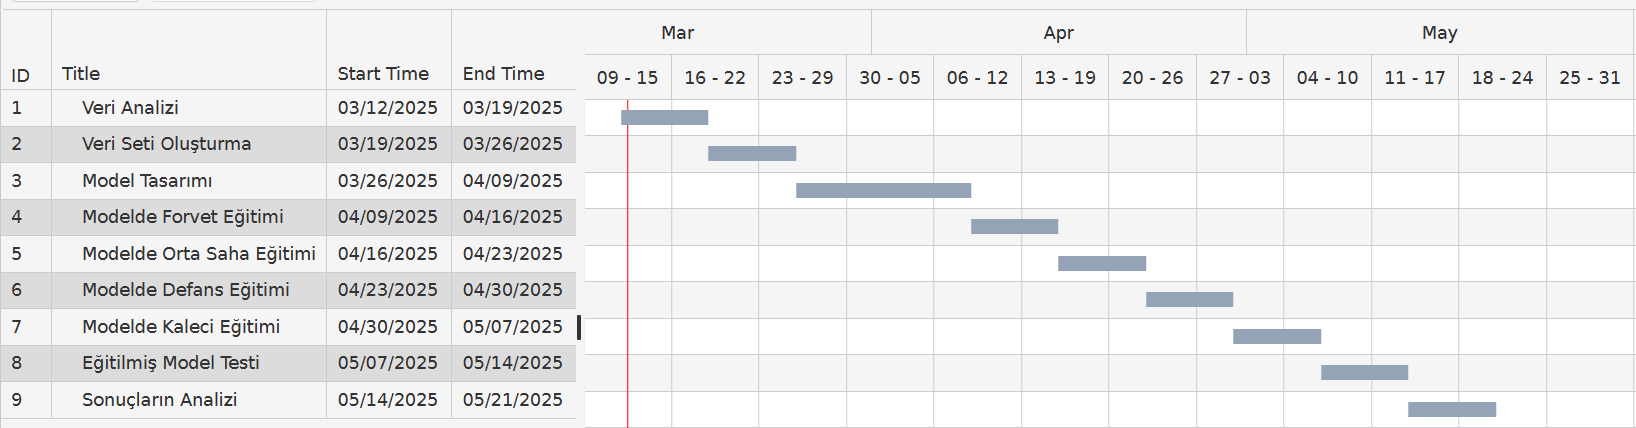
\includegraphics[width=\textwidth]{Chart.png} 
    \caption{Gantt Şeması}
\end{figure}

\renewcommand{\refname}{Kaynakça}
\begin{thebibliography}{9}
\bibitem{transfermarkt}
\href{https://www.transfermarkt.com.tr/}{Transfermarkt}, Futbolcu istatistikleri ve transfer verileri, 2025.

\bibitem{sofascore}
\href{https://www.sofascore.com/tr/}{Sofascore}, Canlı futbol verileri ve oyuncu analizleri, 2025.

\bibitem{fifa}
\href{https://www.fifa.com/}{FIFA}, Uluslararası futbol verileri ve organizasyon bilgileri, 2025.


\bibitem{github1}
G. Ferreiro, \href{https://github.com/gonzaferreiro/Market_value_football_players}{Market Value Football Players}, GitHub repository, 2025.

\bibitem{github2}
Mr. Vaita, \href{https://github.com/mrvaita/footballers_value}{Footballers Value}, GitHub repository, 2025.
\\bibitem{huang2023} 
Huang, J., \& Zhang, W. (2023). "Predicting football player market value using SHAP-based machine learning models." 

 
\bibitem{cgpt}
\href{https://chatgpt.com/c/67cec41b-6bb4-8012-87f6-43de845c25bb}{ChatGpt}, Yapay Zeka Destekli Asistan, OpenAI, 2025.


\end{thebibliography}





\end{document}



